\documentclass{standalone}
\usepackage{tikz}
\usetikzlibrary{patterns, positioning}


\begin{document}
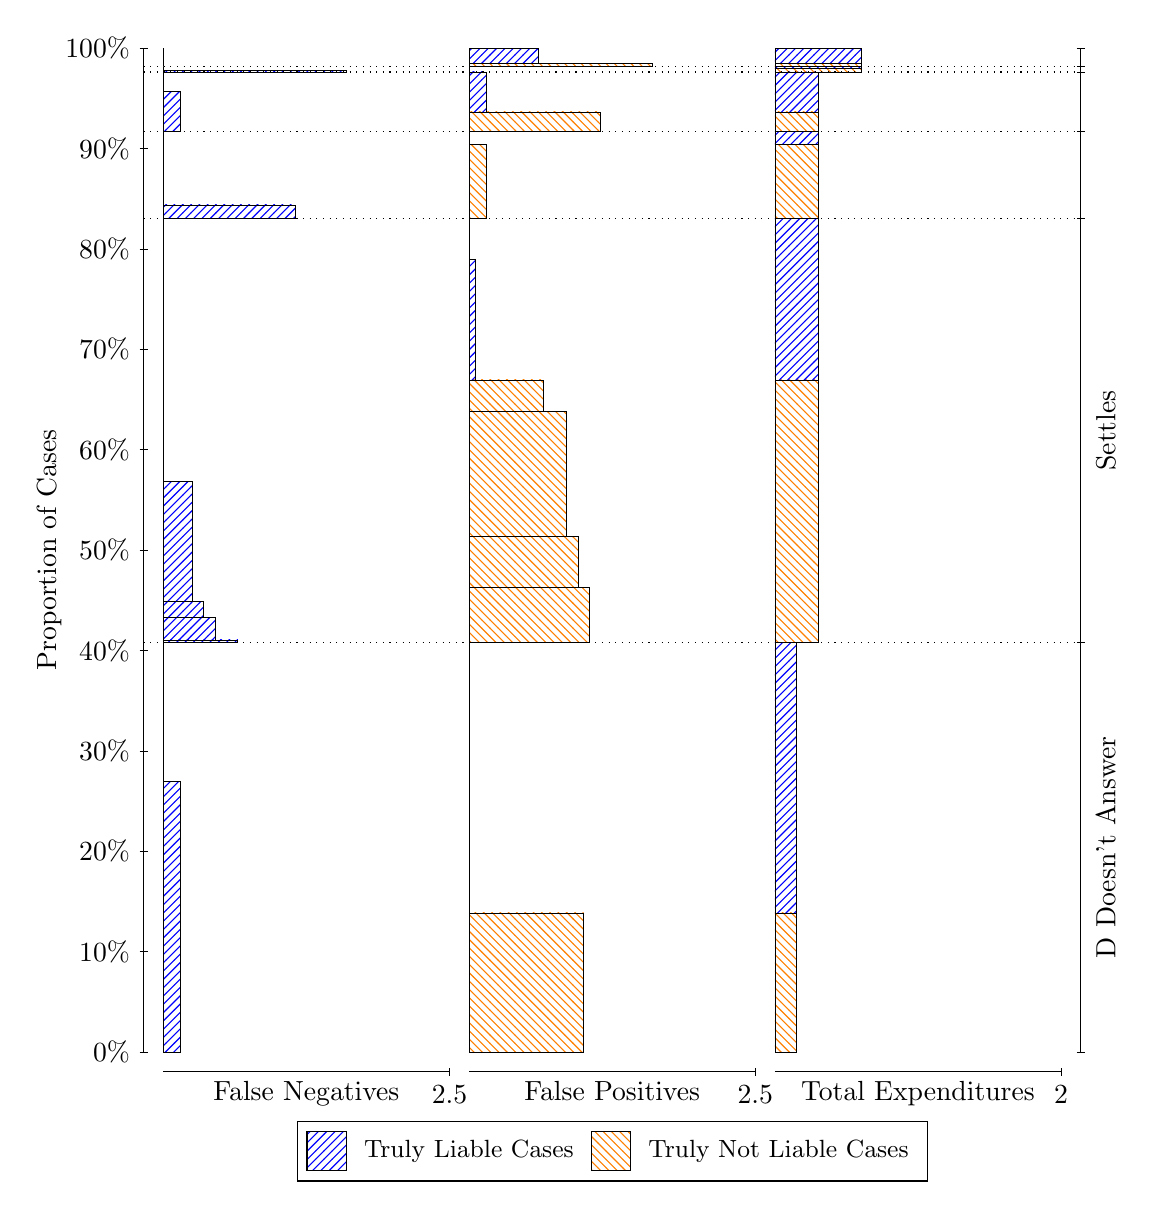
\begin{tikzpicture}
\draw[black, very thin] (1.5,1.75) -- (1.5,14.5);
\node[rotate=90, text=black, anchor=center] at (0.3, 8.125) {Proportion of Cases};
\draw[black, very thin] (1.45,1.75) -- (1.55,1.75);
\node[text=black, anchor=east] at (1.45, 1.75) {0\%};
\draw[black, very thin] (1.45,3.025) -- (1.55,3.025);
\node[text=black, anchor=east] at (1.45, 3.025) {10\%};
\draw[black, very thin] (1.45,4.3) -- (1.55,4.3);
\node[text=black, anchor=east] at (1.45, 4.3) {20\%};
\draw[black, very thin] (1.45,5.575) -- (1.55,5.575);
\node[text=black, anchor=east] at (1.45, 5.575) {30\%};
\draw[black, very thin] (1.45,6.85) -- (1.55,6.85);
\node[text=black, anchor=east] at (1.45, 6.85) {40\%};
\draw[black, very thin] (1.45,8.125) -- (1.55,8.125);
\node[text=black, anchor=east] at (1.45, 8.125) {50\%};
\draw[black, very thin] (1.45,9.4) -- (1.55,9.4);
\node[text=black, anchor=east] at (1.45, 9.4) {60\%};
\draw[black, very thin] (1.45,10.675) -- (1.55,10.675);
\node[text=black, anchor=east] at (1.45, 10.675) {70\%};
\draw[black, very thin] (1.45,11.95) -- (1.55,11.95);
\node[text=black, anchor=east] at (1.45, 11.95) {80\%};
\draw[black, very thin] (1.45,13.225) -- (1.55,13.225);
\node[text=black, anchor=east] at (1.45, 13.225) {90\%};
\draw[black, very thin] (1.45,14.5) -- (1.55,14.5);
\node[text=black, anchor=east] at (1.45, 14.5) {100\%};

\draw[black, very thin] (13.4,1.75) -- (13.4,14.5);
\draw[black, very thin] (13.35,1.75) -- (13.45,1.75);
\node[anchor=west] at (13.35, 1.75) {};
\draw[black, very thin] (13.35,6.9492) -- (13.45,6.9492);
\node[anchor=west] at (13.35, 6.9492) {};
\draw[black, very thin] (13.35,12.338) -- (13.45,12.338);
\node[anchor=west] at (13.35, 12.338) {};
\draw[black, very thin] (13.35,13.444) -- (13.45,13.444);
\node[anchor=west] at (13.35, 13.444) {};
\draw[black, very thin] (13.35,14.196) -- (13.45,14.196);
\node[anchor=west] at (13.35, 14.196) {};
\draw[black, very thin] (13.35,14.268) -- (13.45,14.268);
\node[anchor=west] at (13.35, 14.268) {};
\draw[black, very thin] (13.35,14.5) -- (13.45,14.5);
\node[anchor=west] at (13.35, 14.5) {};

\draw[black, very thin, pattern color=blue, pattern=north east lines] (1.75,1.75) rectangle (1.968,5.1826);
\draw[black, very thin, pattern color=orange, pattern=north west lines] (1.75,5.1826) rectangle (1.75,6.9492);
\draw[black, very thin, pattern color=blue, pattern=north east lines] (1.75,6.9492) rectangle (2.6947,6.9834);
\draw[black, very thin, pattern color=blue, pattern=north east lines] (1.75,6.9834) rectangle (2.404,7.2652);
\draw[black, very thin, pattern color=blue, pattern=north east lines] (1.75,7.2652) rectangle (2.2587,7.4769);
\draw[black, very thin, pattern color=blue, pattern=north east lines] (1.75,7.4769) rectangle (2.1133,9.001);
\draw[black, very thin, pattern color=orange, pattern=north west lines] (1.75,9.001) rectangle (1.75,12.338);
\draw[black, very thin, pattern color=blue, pattern=north east lines] (1.75,12.338) rectangle (3.4213,12.507);
\draw[black, very thin, pattern color=orange, pattern=north west lines] (1.75,12.507) rectangle (1.75,13.444);
\draw[black, very thin, pattern color=blue, pattern=north east lines] (1.75,13.444) rectangle (1.968,13.95);
\draw[black, very thin, pattern color=orange, pattern=north west lines] (1.75,13.95) rectangle (1.75,14.196);
\draw[black, very thin, pattern color=blue, pattern=north east lines] (1.75,14.196) rectangle (4.0753,14.219);
\draw[black, very thin, pattern color=orange, pattern=north west lines] (1.75,14.219) rectangle (1.75,14.268);
\draw[black, very thin, pattern color=orange, pattern=north west lines] (1.75,14.268) rectangle (1.75,14.307);
\draw[black, very thin, pattern color=blue, pattern=north east lines] (1.75,14.307) rectangle (1.75,14.5);
\draw[black, very thin, pattern color=orange, pattern=north west lines] (5.6333,1.75) rectangle (7.0867,3.5167);
\draw[black, very thin, pattern color=blue, pattern=north east lines] (5.6333,3.5167) rectangle (5.6333,6.9492);
\draw[black, very thin, pattern color=orange, pattern=north west lines] (5.6333,6.9492) rectangle (7.1593,7.6492);
\draw[black, very thin, pattern color=orange, pattern=north west lines] (5.6333,7.6492) rectangle (7.014,8.2943);
\draw[black, very thin, pattern color=orange, pattern=north west lines] (5.6333,8.2943) rectangle (6.8687,9.8862);
\draw[black, very thin, pattern color=orange, pattern=north west lines] (5.6333,9.8862) rectangle (6.578,10.286);
\draw[black, very thin, pattern color=blue, pattern=north east lines] (5.6333,10.286) rectangle (5.706,11.811);
\draw[black, very thin, pattern color=blue, pattern=north east lines] (5.6333,11.811) rectangle (5.6333,12.338);
\draw[black, very thin, pattern color=orange, pattern=north west lines] (5.6333,12.338) rectangle (5.8513,13.276);
\draw[black, very thin, pattern color=blue, pattern=north east lines] (5.6333,13.276) rectangle (5.6333,13.444);
\draw[black, very thin, pattern color=orange, pattern=north west lines] (5.6333,13.444) rectangle (7.3047,13.69);
\draw[black, very thin, pattern color=blue, pattern=north east lines] (5.6333,13.69) rectangle (5.8513,14.196);
\draw[black, very thin, pattern color=orange, pattern=north west lines] (5.6333,14.196) rectangle (5.6333,14.245);
\draw[black, very thin, pattern color=blue, pattern=north east lines] (5.6333,14.245) rectangle (5.6333,14.268);
\draw[black, very thin, pattern color=orange, pattern=north west lines] (5.6333,14.268) rectangle (7.9587,14.307);
\draw[black, very thin, pattern color=blue, pattern=north east lines] (5.6333,14.307) rectangle (6.5053,14.5);
\draw[black, very thin, pattern color=orange, pattern=north west lines] (9.5167,1.75) rectangle (9.7892,3.5167);
\draw[black, very thin, pattern color=blue, pattern=north east lines] (9.5167,3.5167) rectangle (9.7892,6.9492);
\draw[black, very thin, pattern color=orange, pattern=north west lines] (9.5167,6.9492) rectangle (10.062,10.286);
\draw[black, very thin, pattern color=blue, pattern=north east lines] (9.5167,10.286) rectangle (10.062,12.338);
\draw[black, very thin, pattern color=orange, pattern=north west lines] (9.5167,12.338) rectangle (10.062,13.276);
\draw[black, very thin, pattern color=blue, pattern=north east lines] (9.5167,13.276) rectangle (10.062,13.444);
\draw[black, very thin, pattern color=orange, pattern=north west lines] (9.5167,13.444) rectangle (10.062,13.69);
\draw[black, very thin, pattern color=blue, pattern=north east lines] (9.5167,13.69) rectangle (10.062,14.196);
\draw[black, very thin, pattern color=orange, pattern=north west lines] (9.5167,14.196) rectangle (10.607,14.245);
\draw[black, very thin, pattern color=blue, pattern=north east lines] (9.5167,14.245) rectangle (10.607,14.268);
\draw[black, very thin, pattern color=orange, pattern=north west lines] (9.5167,14.268) rectangle (10.607,14.307);
\draw[black, very thin, pattern color=blue, pattern=north east lines] (9.5167,14.307) rectangle (10.607,14.5);
\draw[black, dotted] (1.5,6.9492) -- (13.4,6.9492);
\draw[black, dotted] (1.5,12.338) -- (13.4,12.338);
\draw[black, dotted] (1.5,13.444) -- (13.4,13.444);
\draw[black, dotted] (1.5,14.196) -- (13.4,14.196);
\draw[black, dotted] (1.5,14.268) -- (13.4,14.268);
\draw[black, very thin] (1.75,1.5) -- (5.3833,1.5);
\node[text=black, anchor=north] at (3.5667, 1.5) {False Negatives};
\draw[black, very thin] (5.3833,1.45) -- (5.3833,1.55);
\node[text=black, anchor=north] at (5.3833, 1.45) {2.5};

\draw[black, very thin] (5.6333,1.5) -- (9.2667,1.5);
\node[text=black, anchor=north] at (7.45, 1.5) {False Positives};
\draw[black, very thin] (9.2667,1.45) -- (9.2667,1.55);
\node[text=black, anchor=north] at (9.2667, 1.45) {2.5};

\draw[black, very thin] (9.5167,1.5) -- (13.15,1.5);
\node[text=black, anchor=north] at (11.333, 1.5) {Total Expenditures};
\draw[black, very thin] (13.15,1.45) -- (13.15,1.55);
\node[text=black, anchor=north] at (13.15, 1.45) {2};

\node[text=black, centered, rotate=90] at (13.72, 4.3496) {D Doesn't Answer};
\node[text=black, centered, rotate=90] at (13.72, 9.6437) {Settles};





\draw (7.449999999999999,1.5) node[draw=none] (baseCoordinate) {};
\begin{scope}[align=center]
        \matrix[scale=0.5, draw=black, below=0.5cm of baseCoordinate, nodes={draw}, column sep=0.1cm]{
            \node[rectangle, draw, minimum width=0.5cm, minimum height=0.5cm, pattern color=blue, pattern=north east lines] {}; &
            \node[draw=none, font=\small, text=black] (B) {Truly Liable Cases}; &
            \node[rectangle, draw, minimum width=0.5cm, minimum height=0.5cm, pattern color=orange, pattern=north west lines] {}; &
            \node[draw=none, font=\small, text=black] (B) {Truly Not Liable Cases}; \\
            };
\end{scope}

\end{tikzpicture}
\end{document}